% 第1章第6节：Hilbert空间的正交结构（闭子空间的正交投影；正交系与正交基；正交展开与截断误差）。

\section{Hilbert空间的正交结构}
\label{sec:fs-orthogonal}

本节固定一个Hilbert空间$H$，例如$L^2(\mu)$或$\ell^2$，研究两个几何问题：给定一个子空间，能否从中取出离目标最近的分量；能否用一组两两正交的方向给每个元素写出坐标。有限维中的答案是熟悉的，无限维中的新问题是极限是否存在、是否留在子空间里。下一章将把这里的投影看作有界线性算子，本节只建立几何结论。

\subsection{闭子空间的正交投影}
\label{sec:fs-projection}

设$M\subseteq H$是线性子空间，$f\in H$。我们想找$M$中离$f$最近的元素，即达到
\[
 d(f,M)=\inf_{m\in M}\|f-m\|
\]
的$m$。下确界总存在，问题是它能否被$M$中的某个元素取到、取到的元素是否唯一。

\begin{theorem}[闭子空间上的正交投影]
\label{thm:fs-projection}
设$H$为Hilbert空间，$M\subseteq H$为闭线性子空间。则对每个$f\in H$，存在唯一的$m_*\in M$使$\|f-m_*\|=d(f,M)$；并且对$m\in M$，$\|f-m\|=d(f,M)$当且仅当$f-m$与$M$中每个元素正交。
\end{theorem}

\begin{proof}
记$d=d(f,M)$。证明分四步，前两步得到存在性，后两步得到正交刻画与唯一性。

第一步，极小化序列是Cauchy列。取$m_n\in M$使$\|f-m_n\|^2<d^2+1/n$。对$f-m_j$与$f-m_k$使用平行四边形恒等式，
\[
 \|m_j-m_k\|^2=2\|f-m_j\|^2+2\|f-m_k\|^2-4\Bigl\|f-\frac{m_j+m_k}{2}\Bigr\|^2 .
\]
$M$是线性子空间，中点$\tfrac{m_j+m_k}2$在$M$中，所以最后一项的范数平方至少为$d^2$。于是$\|m_j-m_k\|^2<2/j+2/k$，$(m_n)$是Cauchy列。

第二步，极限存在且留在$M$中。$H$完备，所以$m_n$收敛到某个$m_*\in H$；$M$闭，所以$m_*\in M$。由范数的连续性，$\|f-m_*\|=\lim_n\|f-m_n\|=d$。

第三步，最近点的残差与$M$正交。设$m_*$达到$d$，记$r=f-m_*$。任取$m\in M$与实数$t$，$m_*+tm\in M$，所以
\[
 \|r\|^2\leq\|r-tm\|^2=\|r\|^2-2t\langle r,m\rangle+t^2\|m\|^2 .
\]
即$t^2\|m\|^2-2t\langle r,m\rangle\geq0$对所有实数$t$成立。若$\langle r,m\rangle\neq0$，取符号与之相同的足够小的$t$会使左边为负，矛盾；故$\langle r,m\rangle=0$。复Hilbert空间中把$t$换成$t\langle m,r\rangle$即可得到同样的结论。

第四步，正交的残差给出唯一的最近点。设$m_*\in M$满足$f-m_*\perp M$。对任意$m\in M$，$m_*-m\in M$与$f-m_*$正交，由勾股恒等式
\[
 \|f-m\|^2=\|f-m_*\|^2+\|m_*-m\|^2 ,
\]
所以$\|f-m\|\geq\|f-m_*\|$，等号当且仅当$m=m_*$。结合第三步，达到$d$的元素恰好是使残差正交的元素，且只有一个。
\end{proof}

图~\ref{fig:fs-projection-geometry}是这个定理的示意。完备性和闭性在第二步中分工明确：前者保证极小化序列有极限，后者保证极限没有离开$M$。第一步用到了平行四边形恒等式，所以这个论证依赖内积；在一般的Banach空间中，最近点可能不存在，也可能不唯一。

\begin{figure}[!htb]
  \centering
  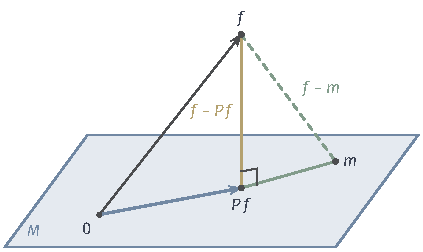
\includegraphics[width=71.7mm]{figures/02-abstract-mathematics/03-function-spaces/tikz/c1-projection-geometry/figure.pdf}
  \caption{闭子空间上的正交投影（示意）。平面代表闭子空间$M$，$Pf$是$M$中离$f$最近的点，残差$f-Pf$与$M$垂直。对$M$中任意另一点$m$，三点构成直角三角形，$\|f-m\|^2=\|f-Pf\|^2+\|Pf-m\|^2$，所以$m$离$f$更远。}
  \label{fig:fs-projection-geometry}
\end{figure}

\paragraph{正交分解与投影的性质}
把定理中的$m_*$记为$P_Mf$，称为$f$在$M$上的\term{正交投影}（orthogonal projection）。记$M^\perp=\{g\in H:\langle g,m\rangle=0\ \text{对所有}\ m\in M\}$为$M$的\term{正交补}（orthogonal complement）。它是闭线性子空间：线性由内积的线性得到，闭性由内积的连续性（Cauchy--Schwarz不等式）得到。定理给出分解
\[
 f=P_Mf+(f-P_Mf),\qquad P_Mf\in M,\quad f-P_Mf\in M^\perp ,
\]
而且这种分解唯一：若$f=m+g=m'+g'$，则$m-m'=g'-g$同时属于$M$与$M^\perp$，与自身正交，只能为零。因此$H=M\oplus M^\perp$。

由正交刻画还可以读出$P_M$的三条性质。线性：$af+bg-(aP_Mf+bP_Mg)=a(f-P_Mf)+b(g-P_Mg)\perp M$，所以$P_M(af+bg)=aP_Mf+bP_Mg$。幂等：$m\in M$时$m$自己就是最近点，$P_M(P_Mf)=P_Mf$。不扩张：由勾股恒等式$\|f\|^2=\|P_Mf\|^2+\|f-P_Mf\|^2$，得$\|P_Mf\|\leq\|f\|$。第~\ref{sec:lfo-self-adjoint}小节将从算子的角度刻画这类映射。

最简单的例子是向常数投影。在$L^2([-1,1])$中取$M=\operatorname{span}\{1\}$，正交条件$\int_{-1}^1(f-c)\,dx=0$给出$c=\tfrac12\int_{-1}^1f\,dx$，即投影是平均值。对$f=x^2$，$P_Mf=\tfrac13$，残差$x^2-\tfrac13$与$1$正交，距离平方为
\[
 \int_{-1}^1\Bigl(x^2-\frac13\Bigr)^2dx=\frac25-\frac49+\frac29=\frac{8}{45} .
\]
这个数在第~\ref{sec:fs-orthonormal-bases}小节的Gram--Schmidt计算中还会出现。

\paragraph{闭性缺失时最近点可能不存在}
定理中的闭性不能去掉。在$H=L^2([-1,1])$中，令$M$为具有连续代表的等价类组成的子空间，它是线性子空间，但由定理~\ref{thm:fs-cc-dense}它在$H$中稠密而不等于$H$，所以不闭。取$f=\operatorname{sgn}$，斜坡给出$\|f-g_n\|_2^2=\tfrac{2}{3n}\to0$，于是$d(f,M)=0$。若下确界被某个$m\in M$取到，则$\|f-m\|_2=0$，$\operatorname{sgn}$与一个连续函数几乎处处相等；而第~\ref{sec:fs-banach}小节已经证明这不可能。所以最近点不存在：每个连续函数都可以再改进，却没有最好的那一个。

本节只处理线性子空间。向一般闭凸集投影时，最近点仍然存在且唯一，但正交条件要换成变分不等式，这与约束优化一起讨论，可参考\BookChapterRef{chap:constrained-optimization}{卷三“有约束优化的求解”章}。

\subsection{正交系与正交基}
\label{sec:fs-orthonormal-bases}

有限维空间中，投影可以用标准正交基的坐标直接写出。现在考察无限多个正交方向。

\begin{definition}[正交归一系]
\label{def:fs-orthonormal}
Hilbert空间$H$中的序列（有限或可数）$(e_j)$称为\term{正交归一系}（orthonormal system），若$\langle e_j,e_k\rangle=\delta_{j,k}$，即两两正交且各自范数为$1$。
\end{definition}

\paragraph{有限个方向上的投影与Bessel不等式}
设$e_1,\ldots,e_m$正交归一，$M_m=\operatorname{span}\{e_1,\ldots,e_m\}$。有限维子空间是闭的（有限维赋范空间完备），所以定理~\ref{thm:fs-projection}适用。记$c_j=\langle e_j,f\rangle$，则
\begin{equation}
 P_{M_m}f=\sum_{j=1}^mc_je_j .
 \label{eq:fs-finite-projection}
\end{equation}
验证只需检查残差：$\langle e_k,f-\sum_jc_je_j\rangle=c_k-c_k=0$对每个$k\leq m$成立，所以残差与$M_m$正交。由勾股恒等式与正交归一性，
\begin{equation}
 \Bigl\|f-\sum_{j=1}^mc_je_j\Bigr\|^2=\|f\|^2-\sum_{j=1}^m|c_j|^2 .
 \label{eq:fs-bessel-error}
\end{equation}

\begin{theorem}[Bessel不等式]
\label{thm:fs-bessel}
设$(e_j)_{j\geq1}$为$H$中的正交归一系，$f\in H$。则$\sum_{j\geq1}|\langle e_j,f\rangle|^2\leq\|f\|^2$。
\end{theorem}

\begin{proof}
由式~\eqref{eq:fs-bessel-error}，左边每个部分和都不超过$\|f\|^2$。非负项级数的部分和有界，级数收敛且和不超过这个界。
\end{proof}

Bessel不等式说明系数平方可和，于是$c_j\to0$：任何元素在越来越靠后的正交方向上的分量都越来越小。

\paragraph{Gram--Schmidt与可数正交基的来源}
正交归一系可以从任意线性无关的序列造出来。设$u_1,u_2,\ldots$线性无关，依次令
\[
 v_k=u_k-\sum_{j<k}\langle e_j,u_k\rangle e_j,\qquad e_k=\frac{v_k}{\|v_k\|} .
\]
$v_k$是$u_k$减去它在$\operatorname{span}\{e_1,\ldots,e_{k-1}\}$上的投影，与之前的方向正交；线性无关保证$v_k\neq0$。归纳可知$\operatorname{span}\{e_1,\ldots,e_k\}=\operatorname{span}\{u_1,\ldots,u_k\}$对每个$k$成立。这就是有限维中的\term{Gram--Schmidt正交化}（Gram--Schmidt orthogonalization），只是现在可以无限地进行下去。

在$L^2([-1,1])$中对$1,x,x^2,x^3$执行这一过程。$e_0=1/\sqrt2$。$x$与$1$正交，$\|x\|^2=\tfrac23$，所以$e_1=\sqrt{3/2}\,x$。对$x^2$，$\langle e_0,x^2\rangle=\tfrac{\sqrt2}3$，$\langle e_1,x^2\rangle=0$，于是$v_2=x^2-\tfrac13$，这正是上一小节向常数投影的残差，$\|v_2\|^2=\tfrac8{45}$，故
\[
 e_2=\sqrt{\tfrac{45}{8}}\Bigl(x^2-\frac13\Bigr)=\sqrt{\tfrac58}\,(3x^2-1).
\]
对$x^3$，它与$e_0,e_2$正交，$\langle e_1,x^3\rangle e_1=\tfrac32\cdot\tfrac25x=\tfrac35x$，于是$v_3=x^3-\tfrac35x$，$\|v_3\|^2=\tfrac27-\tfrac{12}{25}+\tfrac{6}{25}=\tfrac{8}{175}$，故$e_3=\sqrt{7/8}\,(5x^3-3x)$。这些就是归一化的Legendre多项式。图~\ref{fig:fs-legendre-gram-schmidt}对照了正交化前后的函数：(a)中$x^2$与$1$、$x^3$与$x$在大部分区间上走向相近，彼此远不正交；(b)中每个$e_k$恰好比前一个多一次变号。

\begin{figure}[!htb]
  \centering
  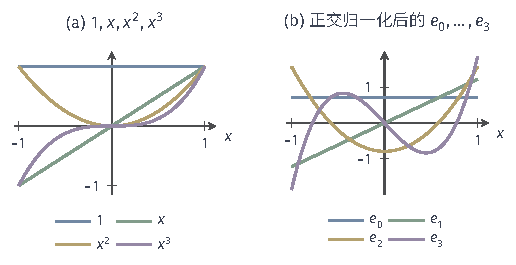
\includegraphics[width=87.3mm]{figures/02-abstract-mathematics/03-function-spaces/tikz/c1-legendre-gram-schmidt/figure.pdf}
  \caption{在$L^2([-1,1])$中对单项式做Gram--Schmidt正交化。(a)$1,x,x^2,x^3$，例如$\langle1,x^2\rangle=\tfrac23\neq0$；(b)得到的$e_0=1/\sqrt2$，$e_1=\sqrt{3/2}\,x$，$e_2=\sqrt{5/8}\,(3x^2-1)$，$e_3=\sqrt{7/8}\,(5x^3-3x)$，两两正交且范数为$1$，$e_k$在$(-1,1)$内恰有$k$个零点。}
  \label{fig:fs-legendre-gram-schmidt}
\end{figure}

同一过程解释了可分Hilbert空间中可数正交归一系的来源。设$H$可分，取可数稠密子集$\{u_k\}$，依次删去能由前面元素线性表出的项，再做Gram--Schmidt，得到正交归一系$(e_j)$，其张成与$\{u_k\}$的张成相同，因而在$H$中稠密。

\paragraph{正交系的完备性}
上面得到的正交系有一个关键性质：它的有限线性组合在$H$中稠密。

\begin{definition}[完备正交系]
\label{def:fs-complete-system}
若正交归一系$(e_j)$的闭线性张成$\overline{\operatorname{span}}\{e_j\}$等于$H$，称它为$H$的\term{完备正交系}（complete orthonormal system），也称\term{标准正交基}（orthonormal basis）。
\end{definition}

这里的“完备”与空间的完备是两个不同的概念：前者说正交系的方向够用，后者说Cauchy列有极限。完备正交系可以用正交性来检验：$(e_j)$完备当且仅当与所有$e_j$都正交的元素只有零。若$(e_j)$完备而$g\perp e_j$对所有$j$成立，则$g$与$\operatorname{span}\{e_j\}$正交，由内积的连续性也与其闭包$H$正交，特别地$\langle g,g\rangle=0$。反之，若闭张成$M\neq H$，取$f\notin M$，由定理~\ref{thm:fs-projection}，$f-P_Mf$是非零元素且与每个$e_j$正交。

\begin{example}[偶方向遗漏奇函数]
\label{ex:fs-even-subspace}
在$L^2([-1,1])$中，偶次的归一化Legendre多项式$e_0,e_2,e_4,\ldots$组成一个无限的正交归一系。但$x$是奇函数，与每个偶函数正交（乘积为奇函数，积分为零），而$x\neq0$，所以这个系不完备。方向有无穷多个，正交性也成立，却仍然遗漏了整个奇函数子空间。

设$E$为几乎处处满足$f(-x)=f(x)$的元素组成的子空间，它是闭的（$L^2$收敛列有几乎处处收敛子列，定理~\ref{thm:fs-ae-subsequence}，极限保持偶性）。任意$f$可以写成$f=\tfrac{f(x)+f(-x)}{2}+\tfrac{f(x)-f(-x)}{2}$，前者是偶函数，后者是奇函数，与$E$正交，所以由定理~\ref{thm:fs-projection}，$P_Ef(x)=\tfrac{f(x)+f(-x)}2$。取$f=e^x$，得$P_Ef=\cosh x$，残差$\sinh x$，见图~\ref{fig:fs-even-odd-projection}；距离平方为$\int_{-1}^1\sinh^2x\,dx=\tfrac{\sinh2}{2}-1\approx0.813$，无论加入多少偶方向都无法减小。
\end{example}

\begin{figure}[!htb]
  \centering
  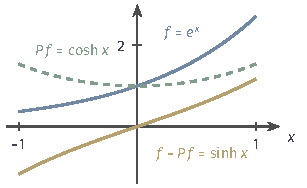
\includegraphics[width=51.9mm]{figures/02-abstract-mathematics/03-function-spaces/tikz/c1-even-odd-projection/figure.pdf}
  \caption{向偶函数子空间的正交投影。$[-1,1]$上$f(x)=e^x$（蓝），投影$Pf=\cosh x$（绿，虚线）为其偶部，残差$f-Pf=\sinh x$（黄）为奇函数，与每个偶函数正交。只用偶方向展开$e^x$时，误差始终至少为$\|\sinh\|_2\approx0.90$。}
  \label{fig:fs-even-odd-projection}
\end{figure}

\subsection{正交展开与截断误差}
\label{sec:fs-orthogonal-expansion}

有了正交归一系，就可以考察无穷级数$\sum_jc_je_j$：它是否收敛，收敛到什么，截断后误差多大。

\begin{theorem}[正交展开与Parseval等式]
\label{thm:fs-parseval}
设$(e_j)_{j\geq1}$为Hilbert空间$H$中的正交归一系，$M=\overline{\operatorname{span}}\{e_j\}$，$f\in H$，$c_j=\langle e_j,f\rangle$。则级数$\sum_jc_je_j$依范数收敛，其和为$P_Mf$。特别地，若$(e_j)$完备，则
\[
 f=\sum_{j=1}^\infty c_je_j\quad(\text{依范数}),\qquad \|f\|^2=\sum_{j=1}^\infty|c_j|^2 .
\]
后一个等式称为\term{Parseval等式}（Parseval identity）。
\end{theorem}

\begin{proof}
记部分和$s_n=\sum_{j\leq n}c_je_j$。对$n>m$，由正交归一性$\|s_n-s_m\|^2=\sum_{m<j\leq n}|c_j|^2$，由Bessel不等式这是收敛级数的一段，所以$(s_n)$是Cauchy列。$H$完备，$s_n$收敛到某个$s$；每个$s_n\in M$而$M$闭，所以$s\in M$。

再验证$f-s\perp M$。对固定的$k$与$n\geq k$，$\langle e_k,f-s_n\rangle=c_k-c_k=0$；令$n\to\infty$，由内积的连续性得$\langle e_k,f-s\rangle=0$。于是$f-s$与$\operatorname{span}\{e_j\}$正交，进而与其闭包$M$正交。由定理~\ref{thm:fs-projection}的正交刻画，$s=P_Mf$。

若$(e_j)$完备，则$M=H$，$P_Mf=f$。在式~\eqref{eq:fs-bessel-error}中令$m\to\infty$，左边趋于$0$，即得Parseval等式。
\end{proof}

对不完备的正交系，展开只恢复$f$在闭张成上的投影，正交补中的分量永远丢失；示例~\ref{ex:fs-even-subspace}中只用偶次Legendre多项式展开$e^x$，奇部$\sinh x$与每个方向都正交，得到的级数和与$e^x$的距离至少为$\|\sinh\|_2$。Bessel不等式与Parseval等式之间的差距，正是这部分丢失的分量。

\paragraph{Legendre多项式的完备性}
判断一个具体的正交系是否完备，需要稠密性论证。对Legendre多项式，三步就够了。由Weierstrass逼近定理，多项式在$(C([-1,1]),\|\cdot\|_\infty)$中稠密；由$\|h\|_2\leq\sqrt2\|h\|_\infty$，一致逼近也是$L^2$逼近；再由定理~\ref{thm:fs-cc-dense}，连续函数在$L^2([-1,1])$中稠密。所以多项式在$L^2([-1,1])$中稠密，而Legendre多项式的张成就是全体多项式，它们组成$L^2([-1,1])$的完备正交系。三角函数系$\{e^{ikx}\}$在$L^2(-\pi,\pi)$中的完备性及傅里叶分析，可参考\BookChapterRef{chap:signal-analysis}{卷三“信号”章}。

\paragraph{截断误差与系数衰减}
固定完备正交系与目标$f$，只改变保留的项数$m$。由式~\eqref{eq:fs-bessel-error}与Parseval等式，
\begin{equation}
 \|f-s_m\|^2=\sum_{j>m}|c_j|^2 ,
 \label{eq:fs-truncation-tail}
\end{equation}
截断误差就是系数平方的尾和。每个$s_m$是$f$在前$m$个方向张成的子空间上的投影，所以在这个子空间内是最好的；但它并没有与其他同样规模的表示比较过，选什么方向是第~\ref{chap:function-approximation}章的问题。

用Legendre多项式展开$\operatorname{sgn}$可以具体看到这些量。$\operatorname{sgn}$是奇函数，只有奇次系数非零；按系数公式精确计算，前几个系数平方为$c_1^2=\tfrac32$，$c_3^2=\tfrac{7}{32}$，$c_5^2=\tfrac{11}{128}$，对应的截断误差$2-\sum_{j\leq m}c_j^2$在$m=1,5,15$时约为$0.500$、$0.195$、$0.077$。图~\ref{fig:fs-legendre-truncation}(a)画出了部分和，(b)把它与$|x|$的展开对照：$|x|$连续，只在$0$处有折角，截断误差下降得快得多，$m=2$时已约为$0.0104$，$m=40$时约为$6\times10^{-6}$；$\operatorname{sgn}$有跳跃，$m=41$时误差仍约为$0.030$。这里只是两个例子的观察；系数衰减与函数光滑性之间的一般关系属于第~\ref{chap:function-approximation}章。

\begin{figure}[!htb]
  \centering
  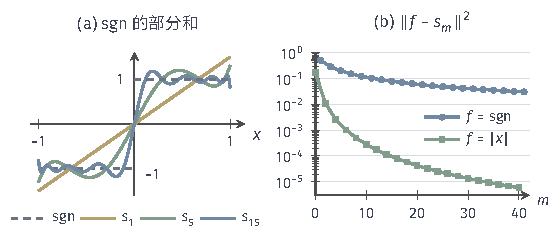
\includegraphics[width=94.9mm]{figures/02-abstract-mathematics/03-function-spaces/tikz/c1-legendre-truncation/figure.pdf}
  \caption{Legendre展开的截断。(a)$\operatorname{sgn}$（虚线）与部分和$s_1,s_5,s_{15}$，其中$s_1=\tfrac32x$；部分和是多项式，在跳跃点附近来回振荡。(b)截断误差$\|f-s_m\|_2^2$（对数纵轴）：$\operatorname{sgn}$取奇数$m$，$|x|$取偶数$m$。两条曲线都单调趋于零，有跳跃的$\operatorname{sgn}$下降慢得多。数值由精确有理运算得到。}
  \label{fig:fs-legendre-truncation}
\end{figure}

\paragraph{从范数收敛到点值收敛}
式~\eqref{eq:fs-truncation-tail}只控制$L^2$误差。图~\ref{fig:fs-legendre-truncation}(a)中的部分和都是连续函数；若它们一致收敛，极限必然连续（定理~\ref{thm:fs-continuous-complete}），而$\operatorname{sgn}$在$0$处跳跃，所以$s_m$不一致收敛到$\operatorname{sgn}$，尽管$L^2$误差趋于零。要从范数收敛得到某点处函数值的收敛，需要“该点的值受范数控制”这样的读取界；$L^2$本身不提供这种界，第~\ref{sec:lfo-point-evaluation}小节将专门讨论这个问题。
